\documentclass[12pt, USenglish]{article}  % Science: US variant of English.

\usepackage{babel}
\usepackage[babel=true]{microtype}
\usepackage[breaklinks, pdfborder={0 0 0}]{hyperref}
\usepackage{csquotes}
\usepackage{amsmath}
\usepackage{units}
\usepackage{tikz}
\usepackage{sansmath}  % Science: sans serif in math in figures.
% Science: Caption labels are boldface "Fig. X." and "Table X.".
\usepackage{caption}
\captionsetup{labelfont=bf, labelsep=period, figurename={Fig.}}
\addto\extrasUSenglish{\renewcommand{\figureautorefname}{Fig.}}

% Setup figure numbering.
\setcounter{figure}{0}

% Science: Prepend 'S' to the appendix number.
\newcommand{\appendixprefix}{S}
\renewcommand{\thefigure}{\appendixprefix\arabic{figure}}


\pagestyle{empty}


\begin{document}

\begin{figure}
  \centering
  \includegraphics{../population_size}
  \caption{The sensitivity of extinction time of FMDV to buffalo
    population size.
    For each model and each SAT, the model was simulated for 1000 runs
    at population sizes 100, 200, 300, 400, 500, 600, 700, 800, 900,
    1000 (baseline, dotted vertical lines), 2000, 3000, 4000, and
    5000.
    The other parameters were fixed at their baseline values.
    The top and middle rows of graphs show the distribution of
    FMDV extinction times for the model with only acute transmission
    and the model with both acute and carrier transmission,
    respectively.
    The bottom row shows the proportion of simulations where FMDV
    persisted in the buffalo population for the whole simulated
    10-year period for the model with both acute and carrier
    transmission.}
\end{figure}


\begin{figure}
  \centering
  \includegraphics{../birth_seasonality}
  \caption{The sensitivity of extinction time to birth seasonality.
    For each model and each SAT, the model was simulated for
    1000 runs at 0, 0.5, 1 (baseline, dotted vertical lines), 1.5, and
    2 times the baseline birth seasonal coefficient of variation of
    0.613.
    The other parameters were fixed at their baseline values.
    The top and middle rows of graphs show the distribution of
    FMDV extinction times for the model with only acute transmission
    and the model with both acute and carrier transmission,
    respectively.
    The bottom row shows the proportion of simulations where FMDV
    persisted in the buffalo population for the whole simulated
    10-year period with both acute and carrier transmission.}
\end{figure}


\begin{figure}
  \centering
  \includegraphics{../samples_sensitivity_acute}
  \caption{The sensitivity of FMDV extinction time to model
    parameters, for the model with only acute transmission.
    The sensitivity is measured by the partial rank correlation
    coefficient (PRCC). The model was simulated with each of 20,000
    samples from the posterior distributions of the parameters
    (Fig.~2, Table S1).}
\end{figure}


\begin{figure}
  \centering
  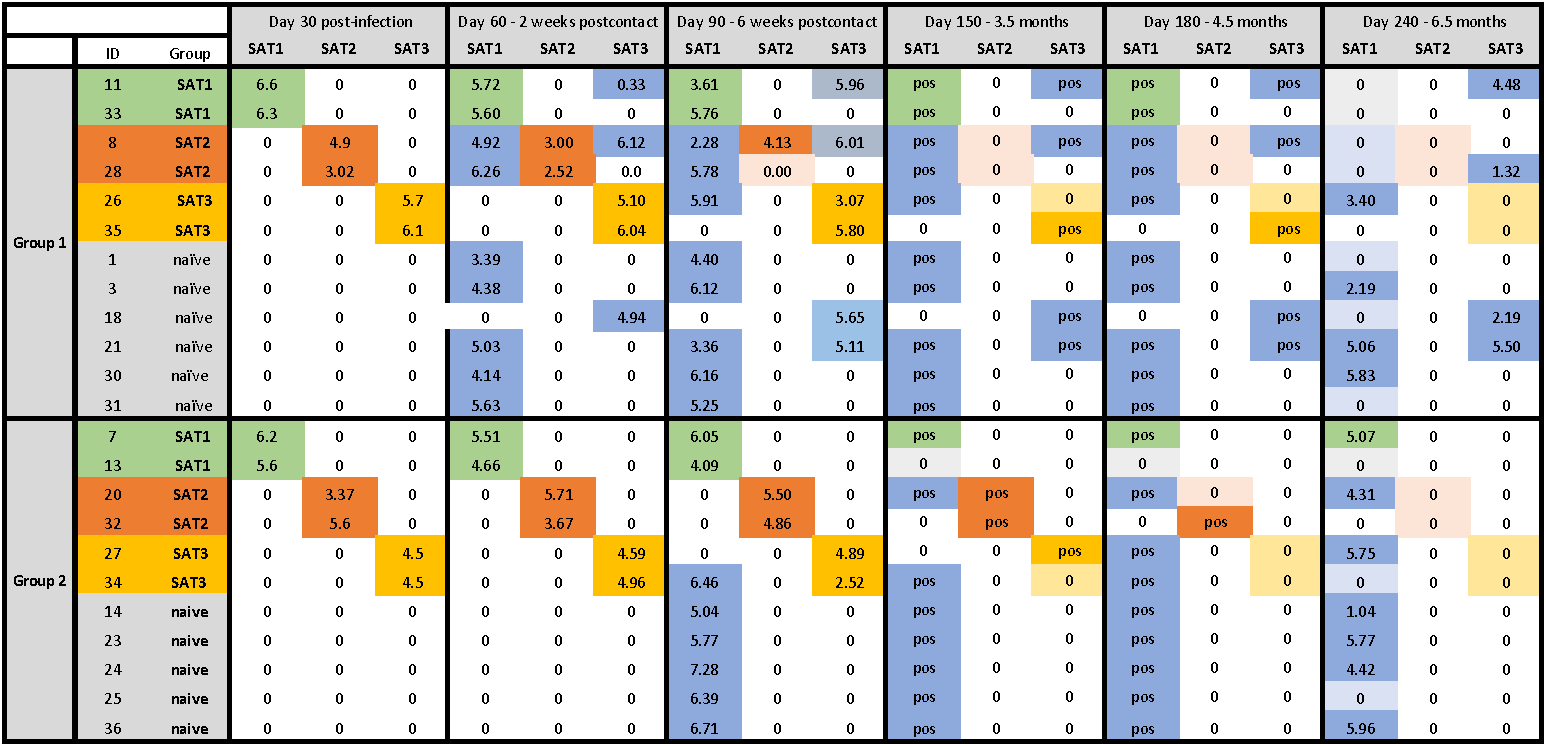
\includegraphics[width=\textwidth]{../transmission_experiment_table}
  \caption{FMDV transmission events from carrier to naïve
    buffalo. Carrier buffalo are shown in green (SAT1), orange (SAT2)
    and yellow (SAT3). Lighter shades indicate loss of carrier status
    in these individuals. Blue shading demarks new infections that
    occurred during the experimental period. The numbers are the log10
    titer of virus genome per \unit{µl} of sample using specific
    primers for each serotype (methods and results described in
    \textit{16}). Samples categorized as positive (pos) were RT PCR
    positive but the Ct value was above a cut off of 32
    (\textit{16}). Carrier status was confirmed on day 30
    post-infection. Experimental groups, each including two carriers
    of each serotype and six naïve buffalo, were assembled on day
    46. All buffalo were sampled for FMDV testing 2 weeks
    post-contact, and subsequently monthly for 6 months. Samples from
    day 120 and day 210 have not been analyzed and are not shown
    here. By two weeks post-contact, at least one transmission event
    from a SAT1 carrier and one from a SAT3 carrier had occurred in
    group one, and by 6 weeks post-contact at least one more
    transmission event from a SAT1 carrier had occurred in group
    2. Additional transmission events may have originated from
    carriers or may reflect secondary infections within each group.}
\end{figure}


\end{document}
